\documentclass[journal]{Imperial_lab_report}


\usepackage{here}
\usepackage{float}
\usepackage{adjustbox}
\usepackage{graphicx}
\usepackage{cite}
\usepackage{amsmath}
\usepackage{amssymb}
\usepackage{pifont}
\usepackage{enumitem}
\usepackage{url}
\usepackage{multirow}
\usepackage{etoolbox}
\usepackage{titlesec}
\newcommand{\cmark}{\ding{51}}

\DeclareMathOperator\erf{erf}

\interdisplaylinepenalty=2500
\hyphenation{op-tical net-works semi-conduc-tor}
\patchcmd{\thebibliography}{\section*{\refname}}{}{}{}
\setcounter{secnumdepth}{4}
\titleformat{\paragraph}
{\normalfont\normalsize\bfseries}{\theparagraph}{1em}{}
\titlespacing*{\paragraph}
{0pt}{3.25ex plus 1ex minus .2ex}{1.5ex plus .2ex}


\begin{document}

\title{Simulation of dust in plasma}
\author{Dogan Akpinar and George E. B. Doran}
\markboth{D. Akpinar \& G. E. B. Doran }
{Shell \MakeLowercase{\textit{et al.}}:}

\maketitle

\begin{abstract}

We have created a simulation that models a spherical dust grain immersed in a plasma and can predict the charge on this dust grain according to various existing charging theories. These theories are the radial motion theory (ABR), orbital motion limited theory (OML) and its derivatives. In our model we have assumed that there is no magnetic field, no external electric field, no collisions and no electron emission of any kind, hence, the simulation is capable of calculating the charge on a dust grain of any size in a plasma of any temperature and flowing at any speed.

\end{abstract}

\section{Introduction}

Plasma is one of four states of matter and makes up over ninety-nine percent of the conventional matter in the universe \cite{99percent}.  Plasma also has a wide range of industrial applications, most notably in semiconductor processing and fusion energy, these applications are highly sensitive to the properties of the plasma. These properties are in turn controlled by the composition of the plasma and the presence of contaminates such as dust and liquid droplets, in this case we take dust to mean any solid particles that can be contained within plasma that are large enough to collect an electric charge \cite{Thomas}. In the semiconductor industry plasmas are used to produce intricate circuit components, vital in the function of electronics, the contamination due to dust particles has lead to a defect rate of around zero point three percent which translates to losses of around one billion dollars a year \cite{Thomas}. In the field of nuclear fusion, a potentially world-changing future source of electrical energy, atoms are heated to extreme temperatures inside a toroidal enclosure called a tokamak, at which point they form plasmas and are collided into each other in an attempt to cause them to fuse and release energy. When the plasma in the tokamak is contaminated by dust, energy can be radiated away from the plasma, fuel can be absorbed away from the plasma and the temperature of the plasma can be reduced to such an extent that the plasma becomes disrupted, which requires the reactor to be turned off, all of which reduce the efficiency of the reactor. This dust can also pose a significant health risk due to toxicity, reactivity or radioactivity \cite{Thomas}.   

\smallskip

In order to predict the influence the dust grains will have on the plasma we must first find the charge it will acquire whilst immersed in the plasma, as the charge dictates the forces that will be exerted on the rest of the plasma and thus how the properties of the plasma will be affected. These predictions will lead to a greater understanding of dust in plasma and allow more effective precautions to be taken in order to reduce the issues discussed. Throughout this report we will describe the way in which we have simulated dust in plasma, which describes plasma with a single dust grain or dust distributed throughout the plasma such that the individual grains do not influence each other. 

\section{Background}

\subsection{Plasma Properties}

\smallskip

A plasma is a gas that has been partially or fully ionised and the behaviour of this gas is dominated by long-range electromagnetic effects \cite{Willis}. Plasmas are neutral macroscopically but microscopically they are composed of positive, negative and in some cases neutral particles. 

\medskip

If we consider a floating wall within a plasma, the floating wall will be charged negatively with respect to its surroundings, until it reaches an equilibrium charge \cite{Willis}. The repulsion of electrons by the negative wall will result in a region of positive space around the wall - known as the sheath. The sheath is usually a few Debye lengths in width, where the Debye length is the distance over which quasi-neutrality breaks down, given by 

\begin{equation}\label{eq:Debye}
\lambda_D = \sqrt{\frac{\varepsilon_{0} k_{B} T_{e}}{n_{0} e^2}},
\end{equation}

\noindent where $\varepsilon_{0}$ is the permittivity of free space, $k_B$ is the Boltzmann constant, $T_e$ is the electron temperature, $n_0$ is the electron density at infinity and $e$ is the electron charge.

\smallskip

Positive ions are continuously absorbed by the negative wall, so there must be a net inward flux of ions into the sheath to maintain the equilibrium; establishing the Bohm criterion, where the speed of the ions required to enter the sheath must be equal to or greater than the cold-ion Bohm speed

\begin{equation}\label{eq:Bohm}
u_{B} = \sqrt{\frac{Z k_{B} T_{e}}{m_{i}}},
\end{equation}

\noindent where $Z$ is the relative ion charge and $m_i$ is the ion mass.

\smallskip

This condition cannot be met by the thermal motion of the ions. Hence, the electric field of the negative wall must extend beyond the sheath, such that the electric field in this region will accelerate the ions so that the Bohm criterion is satisfied - this region beyond the sheath is known as the pre-sheath \cite{Willis}.

\smallskip 

As there is a potential at the surface of the wall and at the sheath edge, there must be a potential drop across the sheath and pre-sheath given as 

\begin{equation}\label{eq:PlanarlimOriginal}
\Delta \phi = \frac{k_B T_e}{2 e}\left(\ln{\left(\frac{2 \pi Z^2}{\mu^2} \right)} - 1\right),
\end{equation}

\noindent normalising and rearranging 

\begin{equation}\label{eq:Planarlim}
{\Delta \Phi = \frac{1}{2}\ln{\left(2 \pi \right)} - \frac{1}{2} - \ln{\left(\frac{\mu}{Z} \right)}},
\end{equation}

\noindent where $\mu = \sqrt{\frac{m_i}{m_e}}$ and $\Delta \Phi = \frac{e \Delta \phi }{k_{B} T_{e}}$ is the normalised potential drop across the sheath and pre-sheath.

\subsection{Quasi-neutrality}

\medskip

Quasi-neutrality refers to two interlinked ideas in physics. The first being the physical observation that if there is a net charged region in the plasma, opposing charges tend to be draw to these regions until the the net charge is neutralised \cite{Thomas}. Secondly, there is the mathematical assumption that positive charge density almost exactly cancels negative charge density \cite{Thomas} 

\begin{equation}\label{eq:Quasi-neutrality}
{Z n_i \approx n_e},
\end{equation}

\noindent where $Z$ is the relative ion charge, $n_i$ is the ion number density and $n_e$ is the electron number density. 

\section{Charging theories}

\subsection{Base assumptions}

Throughout the writing of our simulation we have made certain base assumptions for our plasma model, ensuring the validity of the theories discussed.

\smallskip 

\noindent Firstly, we have assumed that we have a uniform, infinite plasma with no magnetic fields and no external electric fields, hence, the dynamics of the plasma is significantly simplified. Secondly, we have assumed that the plasma is quasi-neutral ensuring that the positive charge density almost exactly cancels the negative charge density given by $Zn_{i} \approx n_{e}$ \cite{Thomas}. Thirdly, we have neglected any thermionic emission of electrons from the dust grain, ensuring that the dust grain can only be charged negatively. Fourthly, we have neglected any collisions between the ions. Finally, we have further assumed that the dust grain remains stationary within the plasma and that the spherical symmetry of the electric field is held for a flowing or static plasma.

\subsection{Orbital-Motion (OM)}

OM theory has the ability to predict the potential of a dust grain and the ion density as a function of radial distance from the dust grain, while accounting for absorption radii. However, the theory is highly complex, leading to unreasonably long computation times when simulating the model \cite{Thomas}. Hence, we use an adapted version of OM known as OML theory, alongside several modifications to OML theory in order to model all possible scenarios of a warm-ion plasma.

\subsection{Orbital-Motion Limited (OML)}

The OML theory of Harold M. Mott-Smith and Irving Langmuir \cite{OriginalOML} models a warm and static plasma, where the kinetic energy of an ion is not neglected and so the motivation behind its equations are built upon the conservation of energy. Our description of OML essentially mirrors the approach of Drew M. Thomas \cite{Thomas} which takes after the approaches of Kennedy and Allen \cite{OML} and Christopher T. N. Willis \cite{Willis}\cite{SandM}.

\smallskip

Firstly, we consider a positive ion of charge $Ze$ and initial speed $v_{0}$ approaching a negatively charged dust grain of charge $Q$ and arbitrary radius $a$ from infinity. We can then define an impact parameter $b$ for the ion which is the perpendicular distance between the ion's initial trajectory and the sphere's centre \cite{Thomas}.

\begin{figure}[H]
\centering
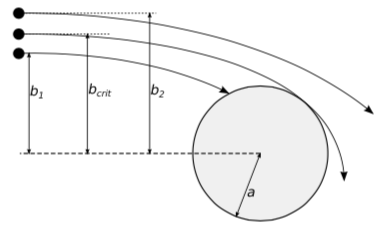
\includegraphics[width=\linewidth]{Output/Impactparameter.jpeg}
\caption{Positive ions approaching a negative dust grain of radius $a$ from infinity, all with initial speed $v_{0}$ but different impact parameters. The ion with impact parameter $b_{crit}$ just grazes the surface of the dust grain, while an ion with impact parameter $b_{1} < b_{crit}$ is collected by the dust grain and an ion with impact parameter $b_{2} > b_{crit}$ escapes the dust grain (Diagram adapted from Thomas \cite{Thomas}).}
\label{OMLtrejectories} 
\end{figure}

If we neglect collisions, we see that the dust grain will absorb an ion depending on its impact parameter and initial speed at infinity. If we consider an ion with initial speed $v_{0}$ and impact parameter $b_{crit}$, then this ion will just graze the surface of the dust grain \cite{Thomas}; while an ion with a smaller impact parameter will be absorbed by the dust grain and an ion with a larger impact parameter will escape the dust grain (Fig. \ref{OMLtrejectories}).

\medskip 

Using conservation of angular momentum and spherical symmetry, we can find an expression for the impact parameter as a function of the the initial speed of the ion and of the tangential speed of the ion as it grazes the sphere's surface. From this expression we can then find a form for the effective cross-section \cite{Thomas}, defined as $\sigma = \pi b_{crit}^2$. As we have neglected collisions we may find an expression for the ion's kinetic energy as it grazes the sphere using the conservation of energy, and by extension find a more sophisticated form for the effective cross-section solely as a function of the initial speed of the ion \cite{Thomas}. By assumption the ions should have a Maxwell-Boltzmann velocity distribution far from the dust grain, hence we may integrate over all possible speeds and so acquire an expression for the ion current

\begin{equation}\label{eq:Icurrent}
I_{i} = 4\pi a^2 n_{i} Ze \sqrt{\frac{k_{B}T_{i}}{2\pi m_{i}}} \left(1 - \frac{Ze\phi_{a}}{k_{B}T_{i}}\right),
\end{equation}

\noindent where $n_{i}$ is the ion number density, $k_{B}$ is the Boltzmann constant, $T_{i}$ is the ion temperature, $m_{i}$ is the ion mass and $\phi_{a}$ is the dust grain surface potential.

\medskip

We may assume that the dust grain always charges negatively \cite{Thomas} and repels any approaching electrons once at equilibrium, hence we can now find a similar expression for the electron current as the electrons obey the Boltzmann relation yielding the following 

\begin{equation}\label{eq:Ecurrent}
I_{e} = -4\pi a^2 n_{0} e \sqrt{\frac{k_{B}T_{e}}{2\pi m_{e}}} \exp\left(\frac{e\phi_{a}}{k_{B}T_{e}}\right),
\end{equation}

\noindent where $n_{0}$ is the electron number density at infinity, $T_{e}$ is the electron temperature and $m_{e}$ is the electron mass.

\smallskip

At equilibrium, $I_{i} + I_{e} = 0$, we can find the steady state solution by equating $I_{i}$ and $I_{e}$, while simultaneously invoking quasi-neutrality to obtain the expression

\begin{equation}\label{eq:OMLeqn}
\frac{\sqrt{\Theta}}{\mu} \left(1 - \frac{Z}{\Theta}\Phi_a \right) \approx \exp{\left(\Phi_a\right)}.
\end{equation}

\medskip

\noindent Solving this equation yields an expression that governs OML theory

\begin{equation}\label{eq:OMLsol}
\Phi_{a} \approx \frac{\Theta}{Z} - W_{0}\left(\frac{\mu\sqrt{\Theta}}{Z} \exp{\left(\frac{\Theta}{Z}\right)}\right),
\end{equation}

\noindent where $Z$ is the relative ion charge, $W_{0}$ is the principal branch of the Lambert W function \cite{Thomas} and the other terms are normalised variables given by 

\begin{equation}\label{eq:Nphi}
\Phi_{a} = \frac{e\phi_{a}}{k_{B}T_{e}},
\end{equation}

\begin{equation}\label{eq:Theta}
\Theta = \frac{T_{i}}{T_{e}}.
\end{equation}

\begin{equation}\label{eq:Mu}
\mu = \sqrt{\frac{m_{i}}{m_{e}}} ,
\end{equation}

\begin{equation}\label{eq:Alpha}
\alpha = \frac{a}{\lambda_d}.
\end{equation}

\medskip

We have produced a program that uses the OML solution to output the normalised surface potential for given values of $\mu$, $\Theta$ and $Z$. 

\begin{figure}[H]
\centering
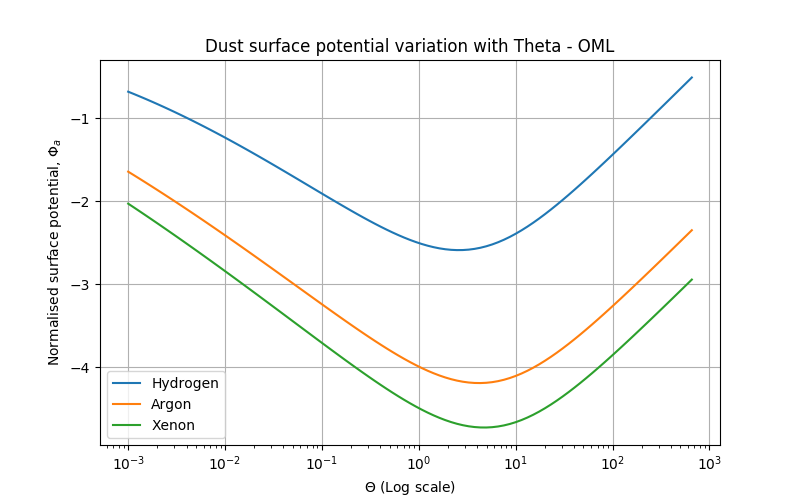
\includegraphics[width=\linewidth]{Output/OMLgraph.jpeg}
\caption{Normalised surface potential as a function of $\Theta$ for singly ionised ($Z = 1$) Hydrogen, Argon and Xenon plasmas according on the OML prediction, plotted on a log-linear scale. The normalised surface potential progressively becomes more negative as the ion species becomes heavier \cite{Thomas}.}
\label{OMLgraph} 
\end{figure}

As the ion species becomes progressively heavier the normalised surface potential becomes more negative, as the Lambert W term in (\ref{eq:OMLsol}) becomes larger. Also, as  $\Theta \xrightarrow{} 0$ the normalised surface potential value also seems to tend to 0 as determined by (\ref{eq:OMLsol}), however as $\Theta$ becomes progressively larger the normalised surface potential becomes more and more negative until reaching a peak value, which seems to be dependant on the ion species; hence, we may conclude that for OML the normalised surface potential is highly dependant on the ion species and the ratio of ion and electron temperatures respectively.  

\smallskip

Allen, Annaratone and de Angelis \cite{Angelis}  show that for a negative charged body in a Maxwellian plasma with $T_{i} \leq T_{e}$ OML is never valid, however, in the limit of small dust grains any error is negligible and so OML is accepted \cite{Willis}. Hence, OML is only valid for a small dust grain and seems to break down at $\alpha_{oml} = 1.25\Theta^{0.4}$ \cite{Willis} for a given $\Theta$ value, where $\alpha = \frac{a}{\lambda_d}$ is the normalised dust grain radius.

\smallskip

Thomas discusses that OML theory guarantee the existence of absorption radii, $r_{A} > a$, such that any ion within $r_{A}$ approaching the dust grain will be absorbed \cite{Thomas}. However, we have decided to neglect the existence of absorption radii as the form of the potential as a function of radial distance from the dust grain centre has a complex and unknown form; hence, neglecting absorption radii allows us to utilise the Debye-Hückle potential which would otherwise be invalid.

\medskip

\subsubsection{Modified OML (MOML)}

\smallskip 

MOML was developed as a modification to OML, such that the theory is applicable to dust grains of larger radii in a static plasma. The fundamental difference in the derivation of MOML compared to OML is that for MOML we apply OML to the spherical boundary between the pre-sheath and sheath surrounding the spherical grain \cite{Thomas}. This establishes the assumption that for $\alpha \xrightarrow{} \infty $ any ion that enters the sheath will eventually be collected by the dust grain. For dust grains of large radii, any absorption radii occur within the sheath, hence, applying OML between the pre-sheath and sheath allows us to eliminate any inaccuracies introduced by such absorption radii \cite{Thomas} \cite{Willis}; ensuring the validity of MOML.

\smallskip

Hence, in equation (\ref{eq:OMLeqn}) we replace $\Phi_a$ with $\Phi_s$, where $\Phi_s$ is the normalised sheath-edge potential. Invoking the large-sphere assumption, quasi-neutrality and the expression for the warm-ion Bohm speed \cite{Thomas}

\begin{equation}\label{eq:WarmBohm}
c_{s} = \sqrt{\frac{k_{B}(T_{e} + \gamma T_{i})}{m_{i}}}.
\end{equation}

\noindent We may find an expression linking $\Phi_a$ with $\Phi_s$

\begin{equation}\label{eq:PhiS}
\Phi_s \approx \Phi_a - \frac{1}{2}\ln{\left[\frac{2\pi Z^2}{\mu^2}(1 + \gamma \Theta)\right]},
\end{equation}

\noindent where $\gamma$ is the heat capacity ratio (adiabatic constant). Substituting (\ref{eq:PhiS}) into the modified (\ref{eq:OMLeqn}) and solving we acquire

\begin{equation}\label{eq:MOMLsol}
\Phi_a \approx  \frac{\Theta}{Z} - W_{0}\left(\sqrt{2\pi \Theta (1 + \gamma \Theta)} \exp{\left (\frac{\Theta}{Z}\right)}\right) + \frac{1}{2}\ln{\left[\frac{2\pi Z^2}{\mu^2}(1 + \gamma \Theta)\right]},
\end{equation}

\noindent which is the MOML solution.

\medskip

Using the equations presented we have then produced a program that follows the same process as the one used for OML but instead is based upon the MOML solution and so is dependant on $\mu$, $\Theta$, $Z$ and $\gamma$ \cite{Coppins}. 

\begin{figure}[H]
\centering
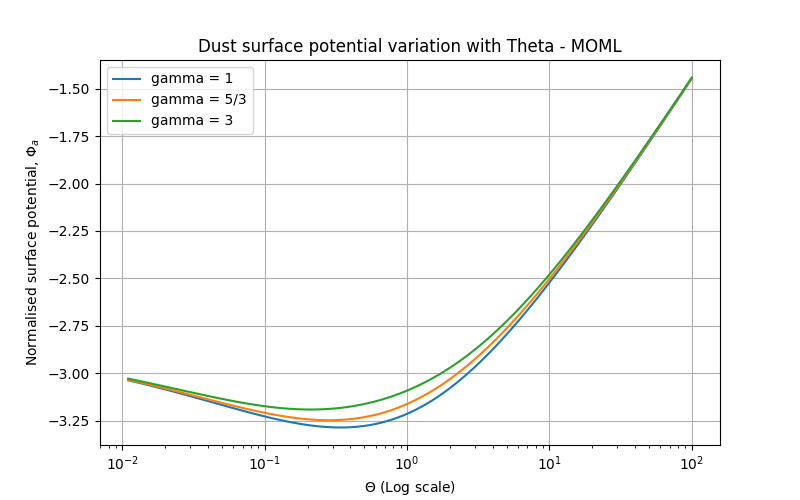
\includegraphics[width=\linewidth]{Output/MOMLgamma.jpeg}
\caption{The MOML prediction for  $\Phi_a$ as a function of $\Theta$, for a hydrogenic ($\mu \approx 43$) and singly ionised ($Z = 1$) plasma with different $\gamma$ \cite{Thomas}.}
\label{MOMLgamma} 
\end{figure}

Willis compares the MOML solution (Fig. \ref{MOMLgamma}) with simulated data ran by the PIC code and concludes that $\gamma = \frac{5}{3}$ seems to produce the most appropriate predictions \cite{Willis}. Hence, $\gamma = \frac{5}{3}$ is chosen as the default heat capacity ratio.

\begin{figure}[H]
\centering
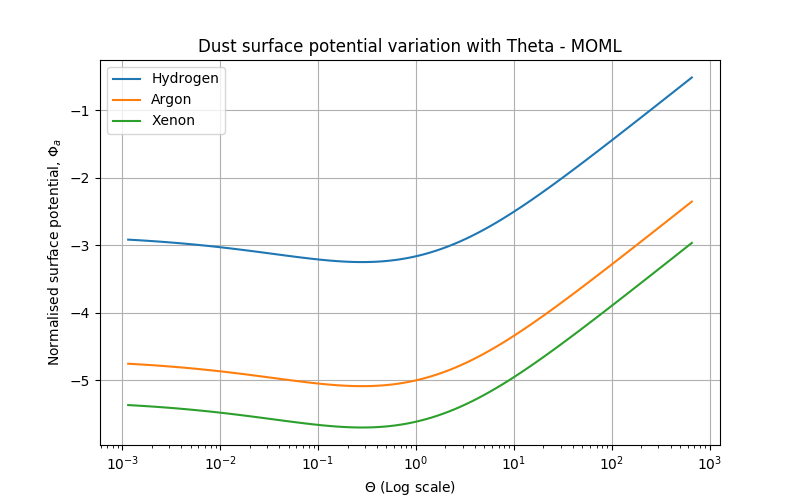
\includegraphics[width=\linewidth]{Output/MOMLgraph.jpeg}
\caption{Normalised surface potential as a function of $\Theta$ for singly ionised ($Z = 1$) Hydrogen, Argon and Xenon plasmas according on the MOML prediction, plotted on a log-linear scale. The normalised surface potential progressively becomes more negative as the ion species becomes heavier \cite{Thomas}.}
\label{MOMLgraph} 
\end{figure}

Just as in the OML model, the normalised surface potential progressively becomes more negative as the ion species becomes heavier. Hence, we may conclude that for the MOML prediction, the normalised surface potential prediction is highly dependant not only on the ion species and $\Theta$ but it is also dependant on the heat capacity ratio, where $\gamma = \frac{5}{3}$ gives the most appropriate predictions \cite{Willis}. From fig. \ref{MOMLgamma} and equation (\ref{eq:MOMLsol}) we see that as $\Theta \xrightarrow{} \infty$ the heat capacity ratio has a negligible effect on the predicted surface potential. 

\medskip

\noindent It should also be noted that unlike the OML prediction, as $\Theta \xrightarrow{} 0$ the predicted $\Phi_a$ is not 0, but instead is 

\begin{equation}\label{eq:MOMlLimNotSimplified}
\lim_{\Theta \to 0} \Phi_a \approx \frac{1}{2}\ln{\left[\frac{2\pi Z^2}{\mu^2}\right]},
\end{equation}e

\noindent which may be further simplified by using the properties of logarithms 

\begin{equation}\label{eq:MOMLlim}
\lim_{\Theta \to 0} \Phi_a \approx \frac{1}{2}\ln{\left(2\pi\right)} - \ln{\left( \frac{\mu}{Z}\right)}.
\end{equation}

\medskip

\subsubsection{Shifted OML (SOML)}

\medskip

A different modification to OML theory produces SOML theory which is used to model the surface potential of a small dust grain in a flowing plasma. The derivation of SOML is identical to that of OML, however, rather than using a static Maxwell-Boltzmann velocity distribution we utilise a flowing Maxwell-Boltzmann velocity distribution \cite{Thomas}. We also further assume that the flow speed is negligible compared to the electron thermal velocity \cite{Thomas} allowing us to equate $I_i$ and $I_e$.

\medskip

Following the derivation and solving analytically in terms of the Lambert W function yields

\begin{equation}\label{eq:SOMLsol}
{\Phi_a \approx \frac{\Theta s_1(\upsilon)}{Z s_2(\upsilon)} - W_0\left(\frac{\mu \sqrt{\Theta}}{Z s_2(\upsilon)} \exp{\left(\frac{\Theta s_1(\upsilon)}{Z s_2(\upsilon)\right)}\right)}},
\end{equation}

\medskip

\noindent where $s_{1}(\upsilon)}$ and $s_{2}(\upsilon)}$ are expressions given by

\begin{equation}\label{eq:S2}
{s_{1}(\upsilon) \equiv  \sqrt{\pi} \frac{\left(1+2\upsilon^2\right) \erf{\left(\upsilon\right)}}{4\upsilon} + \frac{\exp{\left(-\upsilon^2\right)}}{2}},
\end{equation}

\begin{equation}\label{eq:S1}
{s_{2}(\upsilon) \equiv \sqrt{\pi} \frac{\erf{\left(\upsilon\right)}}{2\upsilon}},
\end{equation}

\begin{equation}\label{eq:Erf}
{\erf{\left(\upsilon\right)} = \frac{2}{\sqrt{\pi}} \int_{0}^{\upsilon} \exp{\left(-\zeta^2\right)}  d\zeta},
\end{equation}


\noindent and $\upsilon$ is defined as the normalised plasma flow speed, given by the plasma flow speed divided by $\sqrt{\frac{2 k_{B} T_{i}}{m_{i}}}$ \cite{Thomas}\cite{NormFactor}\cite{NormFactorCoppins}.

\medskip

We have again produced an identical program to OML that instead returns the SOML prediction, we see that the prediction for a small dust grain in a flowing plasma has an additional dependance on the normalised plasma flow speed.

\begin{figure}[H]
\centering
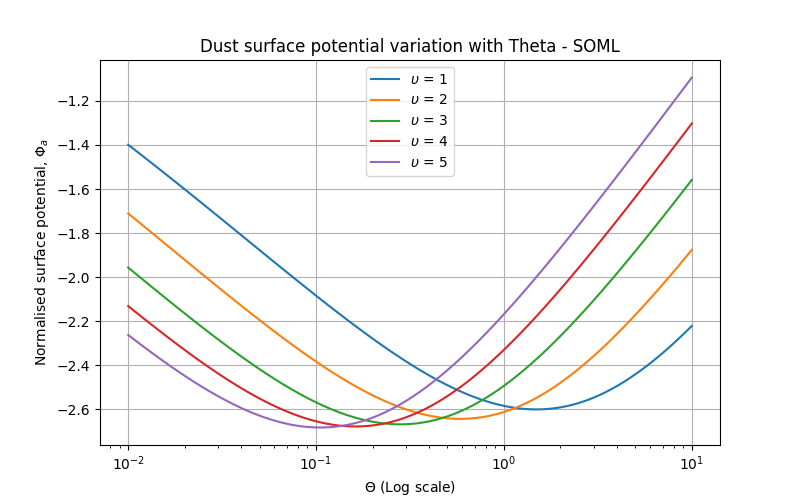
\includegraphics[width=\linewidth]{Output/SOMLgraph.jpeg}
\caption{SOML predictions for $\Phi_a$ as a function of $\Theta$ for a dust grain in a hydrogenic ($\mu \approx 43$) and singly ionised plasma ($Z=1$) with different normalised plasma flow speeds \cite{Thomas}. It seems that as $\upsilon$ increases, the maximum $\Phi_a$ is achieved with a smaller $\Theta$ for a given ion species.}
\label{SOMLgraph} 
\end{figure}

\subsubsection{Shifted, modified OML (SMOML)}

\medskip

Simultaneously implementing the SOML and MOML modifications to OML will produce SMOML theory, where we may model the surface potential of a large dust grain in a flowing plasma. Invoking the modifications to produce MOML and SOML throughout the derivation and solving yields 

\begin{multline}\label{eq:SMOMLsol}
{\Phi_a \approx \frac{\Theta s_{1}(\upsilon)}{Z s_{2}(\upsilon)} - W_{0}\left(\frac{\sqrt{2\pi\Theta\left(1 + \gamma\Theta\right)}}{s_{2}(\upsilon)} \exp{\left(\frac{\Theta s_{1}(\upsilon)}{Z s_{2}(\upsilon)\right)}\right)} \\ + \frac{1}{2}\ln{\left[\frac{2\pi Z^2}{\mu^2}(1 + \gamma \Theta)\right]}}.
\end{multiline}

Using the SMOML solution, we have modelled SMOML using a computer function, producing Fig. \ref{SMOMLgraph}.

\begin{figure}[H]
\centering
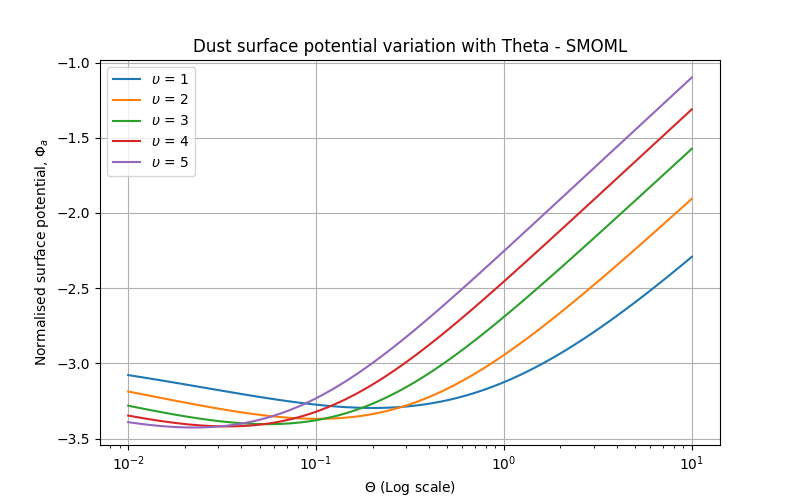
\includegraphics[width=\linewidth]{Output/SMOMLgraph.jpeg}
\caption{SMOML predictions for $\Phi_a$ as a function of $\Theta$ for a dust grain in a hydrogenic ($\mu \approx 43$) and singly ionised plasma ($Z=1$) with different normalised plasma flow speeds \cite{Thomas}.}
\label{SMOMLgraph} 
\end{figure}

\subsubsection{Static numerical fit (SNF)}

\medskip

OML and MOML exist in order to model the potential of dust grains of extreme radii ($ a \xrightarrow{} 0$ and $a \xrightarrow{} \infty$) in a static plasma; however, OML and MOML do not account for intermediate radii. As mentioned in the OML section, OML seems to break down at approximately $\alpha_{oml} = 1.25\Theta^{0.4}$, while Willis discusses that as dust radius increases the potential seems to approach an asymptotic value determined by MOML for finite $\Theta$; this asymptotic value is approached when $\alpha_{moml} \approx 50$ \cite{Willis}.

\smallskip

Hence, for intermediate radii it seems appropriate to implement a numerical fit; Willis discusses this solution and compares it against data points acquired from PIC code \cite{Willis}. He concludes that an appropriate numerical fit is of the following form

\begin{multline}\label{eq:Numfit}
{\Phi_{a}(\alpha) = \left(\frac{\Phi_{moml} - \Phi_{oml}}{\ln{\left(\alpha_{moml}\right)} - \ln{\left(\alpha_{oml}\right)}} \right)\ln{\left(\frac{\alpha}{\alpha_{moml}}\right)} + \Phi_{moml}},
\end{multiline}

\noindent where $\Phi_{oml}$ is the normalised surface potential determined by OML, $\Phi_{moml}$ is the normalised surface potential determined by MOML and $\Phi_{a}$ is defined as the normalised surface potential in the transition region \cite{Willis}.

\smallskip

The program that we have written according to this equation produces a graph of the following form

\begin{figure}[H]
\centering
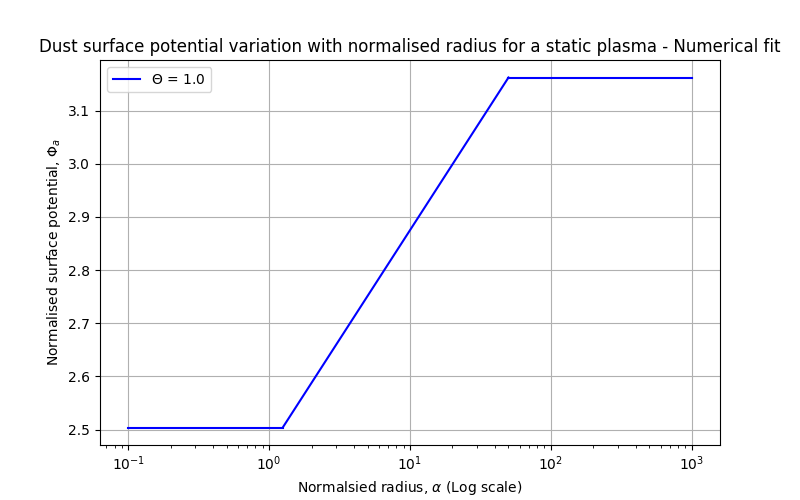
\includegraphics[width=\linewidth]{Output/staticgraph.jpeg}
\caption{Variation of absolute value of $\Phi_a$ with $\alpha$ on a log-linear scale for a static, singly charged ($Z = 1$) hydrogenic ($\mu \approx 43$) plasma setting $\Theta = 1$. The first horizontal line is determined by OML, the linear fit is determined by the numerical fit presented by Willis \cite{Willis} and the second horizontal line is determined by MOML. }
\label{StaticNumFit} 
\end{figure}

\subsubsection{Flowing numerical fit (FNF)}

\medskip

Similarly, SOML and SMOML model the potential of dust grains of extreme radii ($ a \xrightarrow{} 0$ and $a \xrightarrow{} \infty$) in a flowing plasma. However, there seems to be no numerical fit that models the potential for intermediate radii in a flowing plasma; hence, for simplicity we have assumed that such a numerical fit will have an identical form to (\ref{eq:Numfit}).

\smallskip

Our program therefore produces a variation with $\Phi_a$ given by Fig \ref{FlowingNumFit}.

\begin{figure}[H]
\centering
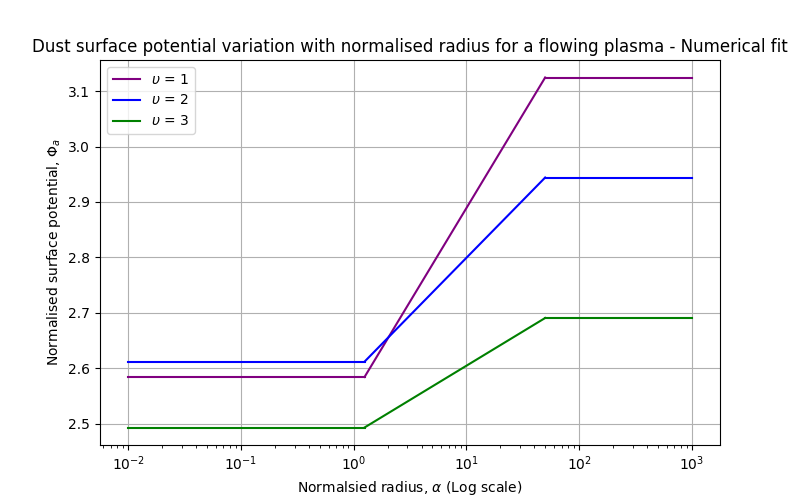
\includegraphics[width=\linewidth]{Output/flowinggraph.jpeg}
\caption{Variation of absolute value of $\Phi_a$ with $\alpha$ on a log-linear scale for a flowing hydrogenic ($\mu \approx 43$) plasma setting $\Theta = 1$, for different normalised plasma flow speeds. The first horizontal line is determined by SOML, the linear fit is determined by the numerical fit presented by Willis \cite{Willis} and the second horizontal line is determined by SMOML.}
\label{FlowingNumFit} 
\end{figure}

\subsection{Allen, Boyd, \& Reynolds (ABR)}

The ABR model is the radial motion theory construced by Allen, Boyd and Reynolds for describing the equilibrium surface potential reached by a dust grain immersed in a plasma \cite{ABR}. The equilibrium surface potential is found by making the assumption that the ions at an infinite distance from the dust grain have no kinetic energy and therefore all the kinetic energy of the ions is due to the potential energy from the dust grain. ABR also assumes that the plasma is collisionless and thus the ions will move radially towards the dust grain, this leads to an expression for the ion current which is entirely dependent on the radial distance from the dust grain, given by

\begin{equation}\label{eq:ABRIi}
{I_i = \frac{4\sqrt{2} \ n_i \pi r^2 Z^{\frac{3}{2}}e^{\frac{3}{2}} \phi_a^{\frac{1}{2}} } {m_i^{\frac{1}{2}}}}.
\end{equation}


As the electrons are faster than the ions, it can be shown that the dust grain will gain a negative charge and thus the potential will be attractive to the ions and repulsive to the electrons, resulting in a limited number of electrons reaching the dust grain and producing a Boltzmann distribution:  

\smallskip

\begin{equation}\label{eq:ABRed}
{n_e(r) = n_0 \exp{\left(\frac{e\phi}{k_B T_e}\right)}},
\end{equation}

assuming that the the dust grain is a perfectly absorbing surface \cite{ABR}. We can assume only inbound electrons contribute to the electron current and consequently it is given by

\begin{equation}\label{eq:ABRIe}
{I_e = 4 \pi a^2 n_0 e \sqrt{\frac{k_B T_e}{2 \pi m_e }} \exp{\left(\frac{e \phi_a}{k_B T_e}\right)}}.
\end{equation}  

It is useful to apply the following normalisations, noting that the same symbol $\Phi$ is now of the opposite sign for simplicity:

\begin{equation}\label{eq:ABRnorm}
{\Phi = - \frac{e\phi}{k_B T_e}}, \ {\rho = \frac{r}{\lambda_D}},\ {\alpha = \frac{a}{\lambda_D}},\ {J = \frac{I_i}{4 \pi \lambda_D^2 n_0 e \sqrt{\frac{2k_B T_e}{m_i}}}}.
\end{equation}

Poisson’s law allows for the formation of a differential equation relating the potential to the difference in the electron and ion densities. By equating expressions for the ion current and electron current in terms of the potential we may form a differential equation in terms of the potential and the distance from the dust grain \cite{ABR}

\begin{equation}\label{eq:ABR9} 
{\frac{d}{d\rho} \left(\rho^2 \frac{d\Phi}{d\rho}\right) = J Z^{-\frac{1}{2}}\Phi^{-\frac{1}{2}}  - \rho^2 \exp{(-\Phi)}}.
 \end{equation}
 
\noindent This equation may be solved using the boundary conditions;

\begin{equation}\label{eq:ABR10}
{ \rho \approx J^{\frac{1}{2}} Z^{-\frac{1}{4}} \Phi^{-\frac{1}{4}} \exp{\left(\frac{\Phi}{2}\right)}},
 \end{equation}
 
 \begin{equation}\label{eq:ABR11}
{\frac{d\Phi}{d\rho}\biggr|_{\rho_b} = \frac{2\rho_b Z^{\frac{1}{2}} J^{-1} \Phi_b^{\frac{3}{2}}}{\Phi_b - \frac{1}{2}} exp{(-\Phi_b)}},
 \end{equation}
 
\begin{equation}\label{eq:ABR13}
{\frac{J}{\Gamma} = \frac{4Z^{\frac{1}{2}}\Phi_b^{\frac{3}{2}}(2\Phi_b - 3)(2\Phi_b + 1)}{(2\Phi_b - 1)^3}},
\end{equation}

\begin{equation}\label{eq:ABR12}
{\frac{J}{\alpha^2} = \frac{\mu}{\sqrt{4\pi}} \exp{\left(-\Phi_a\right)}},
\end{equation}


which are formed by assuming that there exists a certain distance $\rho_b$, past which, quasi-neutrality applies. Where the potential at this point is given by $\Phi_b$, and $\Gamma$ is a number much greater than unity \cite{ABR}. In order to find a value for the surface potential we must solve (\ref{eq:ABR9}), this can only be achieved through use of a numerical method. Initially we choose a value for J, using this and $\Gamma = 10000$ we may find a value for $\Phi_b$ using (\ref{eq:ABR12}), we can then solve for $\rho_b$ and $\frac{d\Phi}{d\rho}\biggr|_{\rho_b}$ using (\ref{eq:ABR10}) and (\ref{eq:ABR11}) respectively. These values form the boundary conditions for (\ref{eq:ABR9}), however we are unable to specify the value of $\alpha$, in order to obtain meaningful information from the solution, we solve  (\ref{eq:ABR9}) simultaneously with (\ref{eq:ABR12}) which yields the pair of values, $\alpha$ and $\Phi_a$ which correspond to the value of J we chose. This is an inconvenient method as we are unable to specify the radius of the dust grain and there is a large computation time, to circumvent this problem we solve the system of equations for a large range of J values and fit a tenth degree polynomial to the data outputted, this allows us to select dust grain radii and obtain the corresponding surface potentials. 

\smallskip

\begin{figure}[H]
\centering
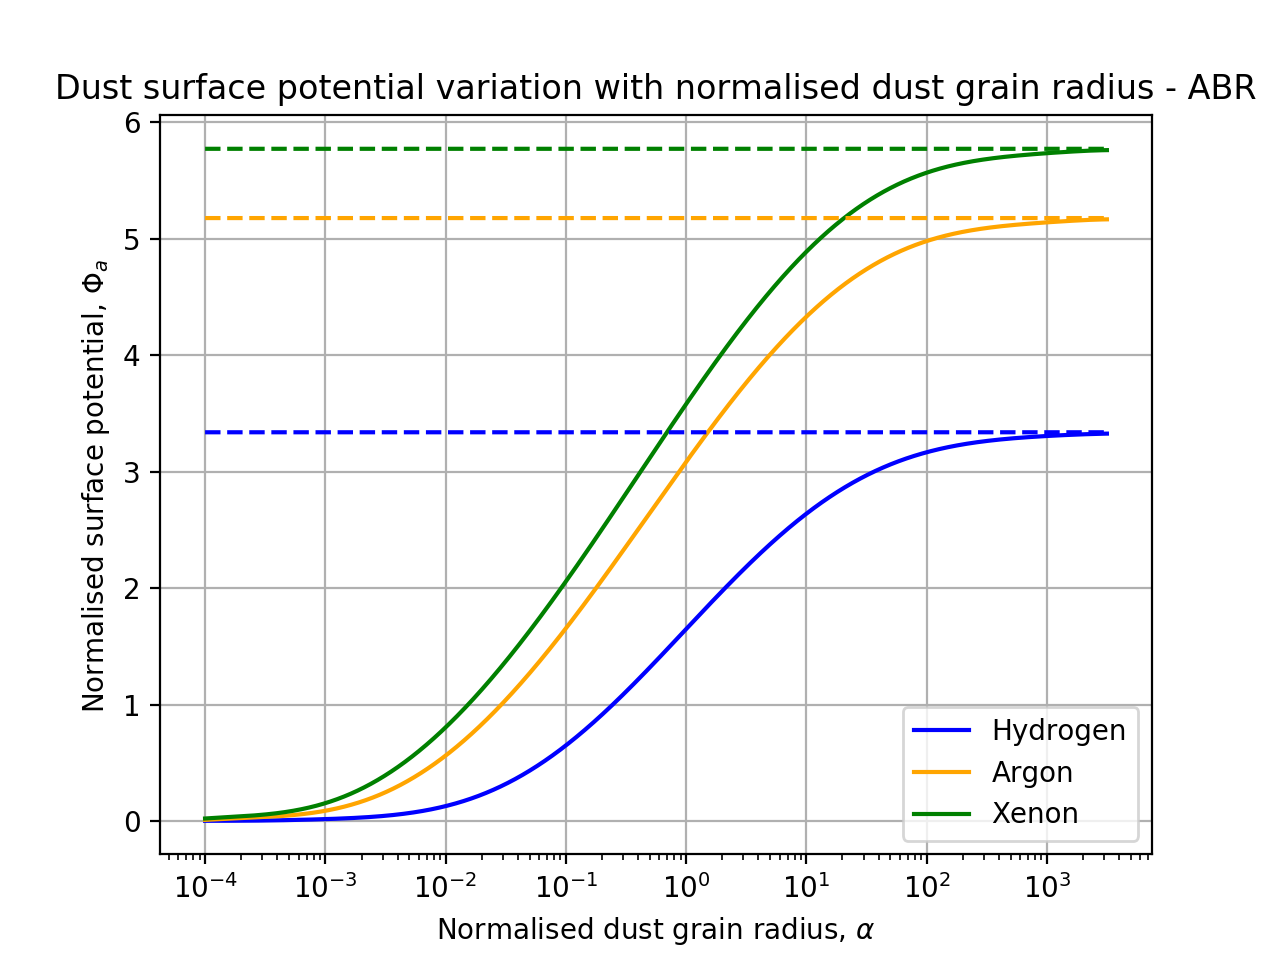
\includegraphics[width=\linewidth]{Output/ABRgraph.jpeg}
\caption{ABR predictions for $\Phi_a$ as a function of $\alpha$ for a dust grain in singly ionised Hydrogen, Argon and Xenon plasmas ($Z=1$) \cite{ABR} \cite{Thomas}.}
\label{ABR} 
\end{figure}

Due to the assumption that the ions have no kinetic energy at infinity ABR theory is restricted to modelling plasmas with ion temperatures significantly lower than the electron temperature, however it is valid for all dust grain radii.

\medskip

\section{Calculating the dust grain charge}

\medskip

We may assume that the variation of potential with radial distance from the dust grain centre is given by the Debye-Hückle potential function 

\begin{equation}\label{eq:DH}
\phi(r) = \frac{Q}{4 \pi \varepsilon_0 r} \exp{\left(\frac{-r}{\lambda_d}\right)},
\end{equation}

\noindent where $Q$ is the dust grain charge, $r$ is the radial distance from the dust grain center and $\lambda_d$ is the Debye length.

\smallskip

Now if we evaluate the Debye-Hückle potential at $r = a$ and rearrange for $Q$ we acquire

\begin{equation}\label{eq:Q}
Q = 4 \pi \varepsilon_0 a \phi_ a  \exp{\left(\frac{a}{\lambda_d}\right)}.
\end{equation}

Using (\ref{eq:Q}) we may calculate the charge on a dust grain given that we know the surface potential of the dust grain. 

\section{Analysis and Results}

\medskip

\subsection{Comparison of OML and ABR at low $\Theta$}

\medskip

We have compared ABR with the OML family for a static plasma as shown by Fig. \ref{OMLvsABR}.

\begin{figure}[H]
\centering
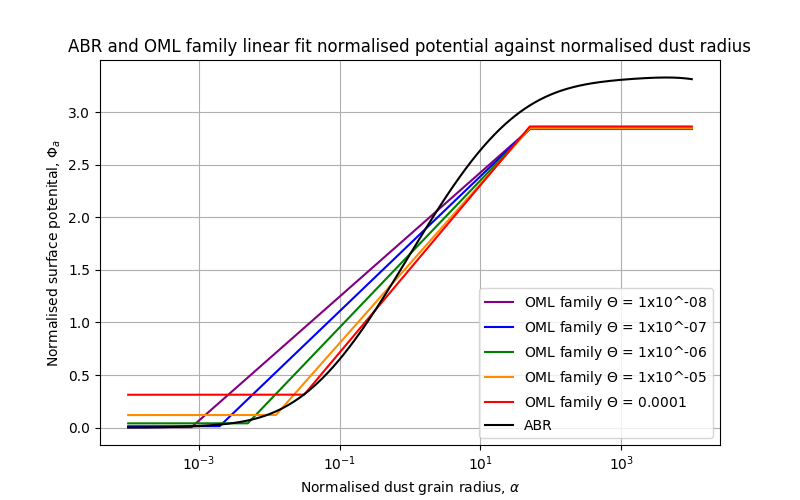
\includegraphics[width=\linewidth]{Output/OMLvsABR.jpeg}
\caption{Variation of absolute value of $\Phi_a$ with $\alpha$ for a flowing hydrogenic ($\mu \approx 43$) plasma on a log-linear scale, comparing ABR to OML, numerical fit and MOML for $\Theta \xrightarrow{} 0$.}
\label{OMLvsABR} 
\end{figure}

\begin{figure}[H]
\centering
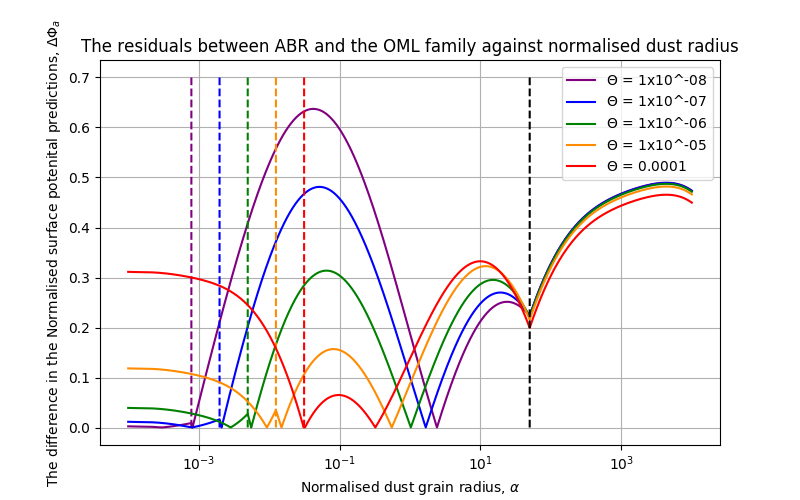
\includegraphics[width=\linewidth]{Output/Residuals.jpeg}
\caption{Residuals between ABR and OML family in the limit of  $\Theta \xrightarrow{} 0$. The coloured vertical lines show the point where OML breaks down for a given $\Theta$, while the black vertical line marks the position where MOML prediction begins.}
\label{Residuals} 
\end{figure}

The comparison shows that as $\Theta \xrightarrow{} 0$ the OML value seems to approach the limit of ABR as $\alpha \xrightarrow{} 0$. We have decided from Fig. \ref{OMLvsABR} that the most appropriate transition $\Theta$ between OML and ABR for our algorithm is $\Theta_{tran} \approx 10^{-5}$.

\smallskip

The numerical fit also seems to break down for $\Theta \xrightarrow{} 0$; plotting the residuals between the graphs implies that the numerical fit deviates from the ABR prediction as shown in Fig. \ref{Residuals}. The peaks corresponding to the numerical fit section of the graph seem to progressively become higher as $\Theta \xrightarrow{} 0$, suggesting that the model deviates even more from ABR as $\Theta$ progressively decreases.

\smallskip

Fig. \ref{OMLvsABR} further shows that the MOML limit does not coincide with the upper ABR limit. The upper ABR limit has the same form as (\ref{eq:Planarlim}) while the MOML limit is given by (\ref{eq:MOMLlim}). Comparing the two limits we see that there is a difference of $\frac{1}{2}$ (\ref{Residuals}), suggesting that MOML intrinsically assumes that there is no potential drop across the pre-sheath; hence, MOML seems to break down as $\Theta \xrightarrow{} 0$. The reason for this is unknown, this may be due to absorption radii beyond the sheath, or the manner in which OML is applied between the pre-sheath and sheath for the derivation of MOML.

\begin{figure}[H]
\centering
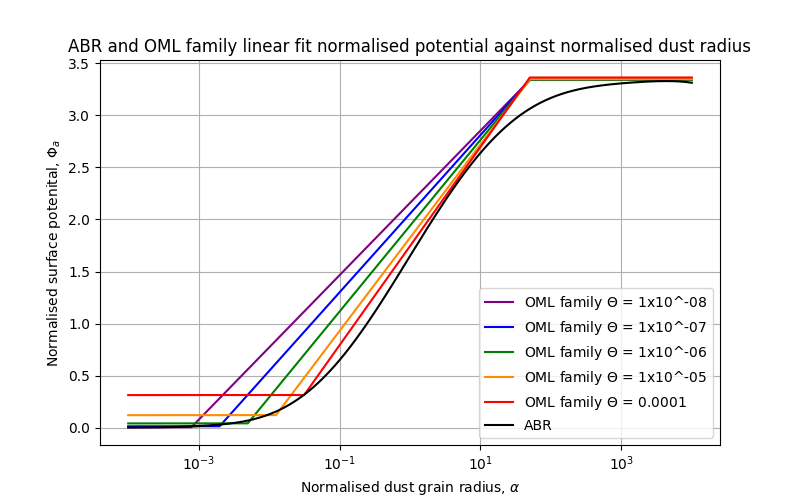
\includegraphics[width=\linewidth]{Output/CorrectedOMLvsABR.jpeg}
\caption{Variation of absolute value of $\Phi_a$ with $\alpha$ for a flowing hydrogenic ($\mu \approx 43$) plasma on a log-linear scale, comparing ABR to OML, numerical and MOML for $\Theta \xrightarrow{} 0$. In this case the MOML limit has been corrected by the subtraction of $\frac{1}{2}$.}
\label{CorrectedOMLvsABR} 
\end{figure}

\begin{figure}[H]
\centering
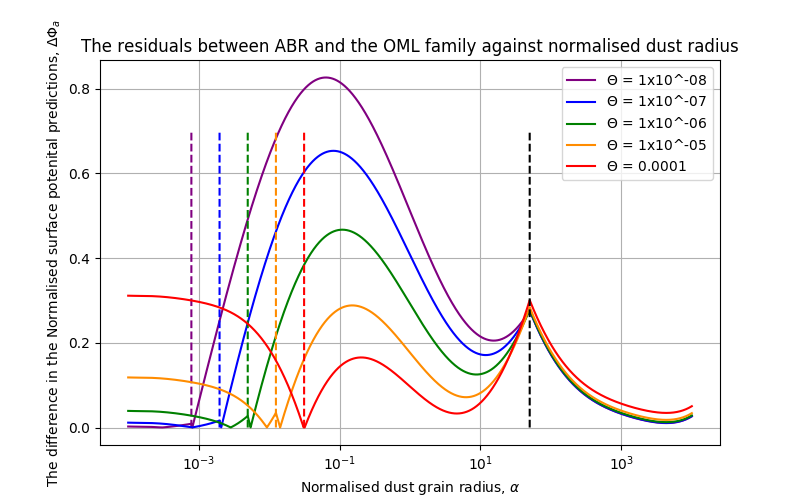
\includegraphics[width=\linewidth]{Output/CorrectedResiduals.jpeg}
\caption{Residuals between ABR and OML family in the limit of  $\Theta \xrightarrow{} 0$, with the corrected MOML limit. The coloured vertical lines show the point where OML breaks down for a given $\Theta$, while the black vertical line marks the position where MOML prediction begins.}
\label{CorrectedResiduals} 
\end{figure}

It is possible to implement a correction to the MOML limit so that it coincides with the upper ABR limit; such a correction could be made by subtracting $\frac{1}{2}$ from the MOML limit, which in turn adjusts the graph as shown by Fig. \ref{CorrectedOMLvsABR}.

\smallskip

The corrected MOML limit seems to almost perfectly coincide with the upper ABR limit for a plasma composed of any element species (any $\mu$). This correction allows MOML to take into account a potential drop across the sheath. However, the correction is solely for the sake of analysis and has no rigorous proof, hence, we have neglected it in our program.

\smallskip

The correction to MOML seems to also affect the numerical fit as seen by the residuals in Fig. \ref{CorrectedResiduals}. The peaks follow the same pattern as stated before, however, they are higher, implying that in this portion of the graph the numerical fit deviates even more than before. As the graph approaches the transition to MOML (region of $\alpha \approx 10^{-1}$ to $50$) the residuals are greatly improved compared to Fig. \ref{Residuals}, suggesting that the numerical fit becomes slightly more accurate for $\Theta \xrightarrow{} 0$ with the possible correction for the MOML limit.


\section{Algorithm}

We have created two scripts, one that finds the charge on the dust grain and the other that outputs a graph according to the chosen model.

\smallskip

ABR is incapable of modelling a flowing plasma. Hence, for the purpose of our simulation, we have assumed that SOML, FNF and SMOML is valid for $\Theta \xrightarrow{} 0$; allowing us to model a flowing cold-ion plasma. However, we are unsure of the accuracy of this model.

\smallskip

Our charge calculating algorithm will ask the user a series of inputs so that it may determine which model should be used under given conditions. The inputs asked are the following: species of the plasma; charge on ion; ion temperature; electron temperature; electron density at infinity; dust grain radius and finally the plasma flow speed. These inputs will then be analysed by the algorithm and trip the required conditional statement depending on the combination of input values, as shown in the table below

\begin{center}
\begin{adjustbox}{width = \columnwidth}
\begin{tabular}{|c|c|c|c|c|c|c|c|} 
\hline
& OML& SNF & MOML & SOML &FNF&SMOML& ABR\\
\hline
 $\Theta \geq 10^{-4}$&\cmark&\cmark&\cmark&\cmark&\cmark&\cmark&\\
\hline
 $\alpha \leq 1.25\Theta^{0.4}$ &\cmark&&&\cmark&&&\cmark\\
\hline
 $1.25\Theta^{0.4} < \alpha <50$ &&\cmark&&&\cmark&&\cmark\\
\hline
$\alpha \geq 50$ &&&\cmark&&&\cmark&\cmark\\
\hline
$\upsilon > 0$  &&&&\cmark&\cmark&\cmark&\\
\hline
\end{tabular}
\end{adjustbox}
\end{center}

\medskip 

\noindent the algorithm will the output the un-normalised dust surface potential and the charge on the dust grain.

\medskip

The graphing algorithm will ask the user for the plasma species, ion charge and what model they wish to graph; depending on the model chosen $\Theta$ will also be asked. The possible output graphs are identical to the graphs presented for each model in the charging theories section, with an additional graph for the SOML and SMOML models.

\section{Conclusion}

We have investigated ABR along with OML and its derivatives to document their validity for given conditions, in order to create a simulation that models a spherical dust grain immersed in plasma and predicts the equilibrium charge that it accumulates. We have assumed that there is no magnetic field, no external electric field, no collisions and no electron emissions of any kind, allowing the charge on a dust grain to be found in a plasma of any temperature, flowing at any rate and containing dust grains of any size using the most appropriate theory available. 
\smallskip

Currently we are unsure of the accuracy of the theories, and by extension, the model. Therefore to ensure the accuracy of the model, the model can be checked with OM theory however this is not always feasible, so experiments could be conducted to measure the charge on the dust grains in plasmas under varying conditions to test the validity of the model.

\smallskip

Due to the discrepancy between the ABR and MOML in the low $\Theta$ limit, further investigation is warranted to ensure that MOML is accurate.

\smallskip

The next logical extension of the model is to incorporate a magnetic field, an external electric field, collisions and account for various types of electron emission.


\section{References and Acknowledgements}
\bibliography{DustyLib}
\bibliographystyle{IEEEtran}

\section{Appendix}

\subsection{Model summary}

\medskip

Base assumptions (valid for all model):

\medskip

\begin{itemize}
\item Spherical symmetry of electric field
\item No collisions
\item No magnetic field
\item No external electric field
\item No electron emission of any kind 
\item Quasi-neutrality in the bulk plasma
\end{itemize}

\medskip

\subsubsection{OML}

\medskip

Assumptions:

\medskip

\begin{itemize}
\item Conservation of particle energy
\item Conservation of particle angular momentum
\item The limiting trajectory is the grazing incidence 
\end{itemize}

\medskip

Validity:

\medskip

\begin{itemize}
\item Any $\Theta$
\item Small $\alpha$ ($\alpha_{oml} \leq 1.25\Theta^{0.4}$)
\item Static plasma
\end{itemize}

\medskip

\subsubsection{MOML}

\medskip

Assumptions:

\medskip

\begin{itemize}
\item Conservation of particle energy
\item Conservation of particle angular momentum
\item Apply OML between dust grain surface and sheath-edge
\end{itemize}

\medskip

Validity:

\medskip

\begin{itemize}
\item Any $\Theta$
\item Large $\alpha$ ($\alpha_{moml} \geq 50$)
\item Static plasma
\end{itemize}

\medskip

\subsubsection{SOML}

\medskip

Assumptions:

\medskip

\begin{itemize}
\item Conservation of particle energy
\item Conservation of particle angular momentum
\item Apply flowing Maxwell-Boltzmann velocity distribution 
\end{itemize}

\medskip

Validity:

\medskip

\begin{itemize}
\item Any $\Theta$
\item Small $\alpha$ ($\alpha_{oml} \leq 1.25\Theta^{0.4}$)
\item Flowing plasma 
\end{itemize}

\medskip

\subsubsection{SMOML}

\medskip

Assumptions:

\medskip

\begin{itemize}
\item Conservation of particle energy
\item Conservation of particle angular momentum
\item Apply OML between dust grain surface and sheath-edge
\item Apply flowing Maxwell-Boltzmann velocity distribution 
\end{itemize}

\medskip

Validity:

\medskip

\begin{itemize}
\item Any $\Theta$
\item Large $\alpha$ ($\alpha_{moml} \geq 50$)
\item Flowing plasma 
\end{itemize}

\medskip

\subsubsection{SNF}

\medskip

Assumptions:

\medskip

\begin{itemize}
\item Conservation of particle energy
\item Conservation of particle angular momentum
\item Apply OML between dust grain surface and sheath-edge
\end{itemize}

\medskip

Validity:

\medskip

\begin{itemize}
\item Any $\Theta$
\item Intermediate $\alpha$ ($1.25\Theta^{0.4} < \alpha < 50$)
\item Static plasma
\end{itemize}

\medskip

\subsubsection{FNF}

\medskip

Assumptions:

\medskip

\begin{itemize}
\item Conservation of particle energy
\item Conservation of particle angular momentum
\item Apply OML between dust grain surface and sheath-edge
\item Apply flowing Maxwell-Boltzmann velocity distribution 
\end{itemize}

\medskip

Validity:

\medskip

\begin{itemize}
\item Intermediate $\alpha$ ($1.25\Theta^{0.4} < \alpha <50$)
\item Flowing plasma 
\end{itemize}

\medskip

\subsubsection{ABR}

\medskip

Assumptions:

\medskip

\begin{itemize}
\item The kinetic energy of ions at infinity is zero
\item A perfectly absorbing surface
\item Beyond a distance $\rho_b$ quasi-neutrality applies
\end{itemize}

\medskip

Validity:

\medskip

\begin{itemize}
\item Very small $\Theta$ ($\Theta < 10^{-4}$)
\item Any $\alpha$
\item Static plasma
\end{itemize}

\subsection{Symbol dictionary}
\begin{center}
\begin{tabular}{cl} 

$e$ & Electron charge \\
$\varepsilon_0$ & Permittivity of free space \\
$k_B$ & Boltzmann's constant \\
$a$ & Dust radius\\
$\alpha$ & Normalised dust radius \\
$_a$ & Subscript indicating a quantity at the dust grain surface \\
$r$ & Distance from the centre of the dust grain \\
$\rho$ & Normalised distance from the centre of the dust grain \\
$\lambda_D$ & Debye length \\
$m_j$ & Mass \\
$n_j$ & Density \\
$T_j$ & Temperature \\
$I_j$ & Current \\
$_j$ & Subscript indicating a plasma particle \\
$_i$ & Subscript indicating an ion quantity \\
$_e$ & Subscript indicating an electron quantity \\
$_0$ & Subscript indicating an electron quantity at infinity \\
$\mu$ & Root mass ratio\\
$\Theta$ & Ratio of ion to electron temperature \\
$\gamma$ & Heat capacity ratio \\
$u$ & Flow velocity \\
$\upsilon$ & Normalised flow velocity \\
$\Gamma$ & ABR correction factor \\
$Z$ & Ion charge number \\
$Q$ & Dust grain charge \\
$\phi$ & Electric potential \\
$\Phi$ & Normalised electric potential \\

\end{tabular}
\end{center}

\end{document}